\documentclass[11pt]{article}
\usepackage{geometry}                % See geometry.pdf to learn the layout options. There are lots.
\geometry{a4paper}                   % ... or a4paper or a5paper or ... 
\usepackage{graphicx}
\usepackage{epstopdf}
\usepackage[unicode]{hyperref}
\usepackage[slovene]{babel}
\usepackage[utf8x]{inputenc}
\usepackage{listings}
\usepackage{xcolor}
\usepackage{textcomp}
\usepackage{multicol}
\usepackage{float}

\DeclareGraphicsRule{.tif}{png}{.png}{`convert #1 `dirname #1`/`basename #1 .tif`.png}
\renewcommand{\baselinestretch}{1.1} % za boljšo berljivost večji razmak
\graphicspath{images/}

\lstset{basicstyle=\ttfamily,
  showstringspaces=false,
  commentstyle=\color{red},
  keywordstyle=\color{blue},
  frame=single
}

\title{Analiza zmogljivosti oblačnih storitev za hranjenje podatkov}
\author{Aleksandar Gogov, Staš Hvala, Matic Repše}
\date{\today}   

\begin{document}
\maketitle


\clearpage
\tableofcontents
\clearpage

\section{Predstavitev ideje}
Lokalni prostor izgublja na pomembnosti, ker se uporabniki vedno pogosteje poslužujejo oblačnega hranjenja podatkov. Osnovne oz. minimalne storitve so po večini brezplačne, možno pa je tudi nadgraditi prostor in uporabljati plačljive storitve, ki uporabniku omogočajo uporabo dodatnih funkcionalnosti. Namen naše raziskovalne naloge je bil testirati najpopularnejše ponudnike (Google Cloud Storage, Amazon S3, Microsoft Azure) in bralcu predstaviti rezultate in ugotovitve testiranj. Naša želja je tudi odkriti, kdo ima zanesljivejšo ter zmogljivejšo performanco oblaka.

\section{Rešitev problema}
Testiranja smo se najprej lotili z CloudHarmony benchmark-om \cite{cloudharm}, da lahko postavimo začetne hipoteze in dobimo okvirno sliko rezultatov. Ker pa nam je konec koncev najpomembnejša neposredna izkušnja uporabnika, smo se odločili, da preverimo kakovost storitev tudi z lastnimi testi (glej poglavje \ref{lastni_testi}) in tako pridemo do pristnejših rezultatov vsakdanje uporabe. Prav tako nam dovoljujejo tudi večjo manipulacijo z bremenom (tip, velikost, število).

\section{CloudHarmony Benchmark} \label{cloudharmony}
CloudHarmony zagotavlja objektivno, nepristransko in zanesljivo analizo uspešnosti za primerjavo storitev računalništva v oblaku. Testirali smo Google Cloud Storage, Amazon S3 in Microsoft Azure v različnih regijah.\\
Osredotočili smo se na dva različna testa:
\begin{itemize}
    \item Downlink
    \begin{itemize}
        \item Downlink [256KB - 10MB / 2 threads],
        \item Downlink [1 - 128KB / 4 threads],
    \end{itemize}
    \item Latency.
\end{itemize}

Na vsako uro smo pognali 6 testov na HTTP protokolu, ker je hitrejši brez dodatnih varnostnih rokovanj.
Kot je bilo pričakovano glede na naš geografski položaj, naši rezultati kažejo najboljšo odzivnost in hitrost prenosa pri evropskih strežnikih. Naše meritve so bile opravljene na 33 različnih točkah, ki so bile porazdeljene na treh kontinentah (US, EU, ASIA). 

\begin{figure}[H]
    \begin{center}
        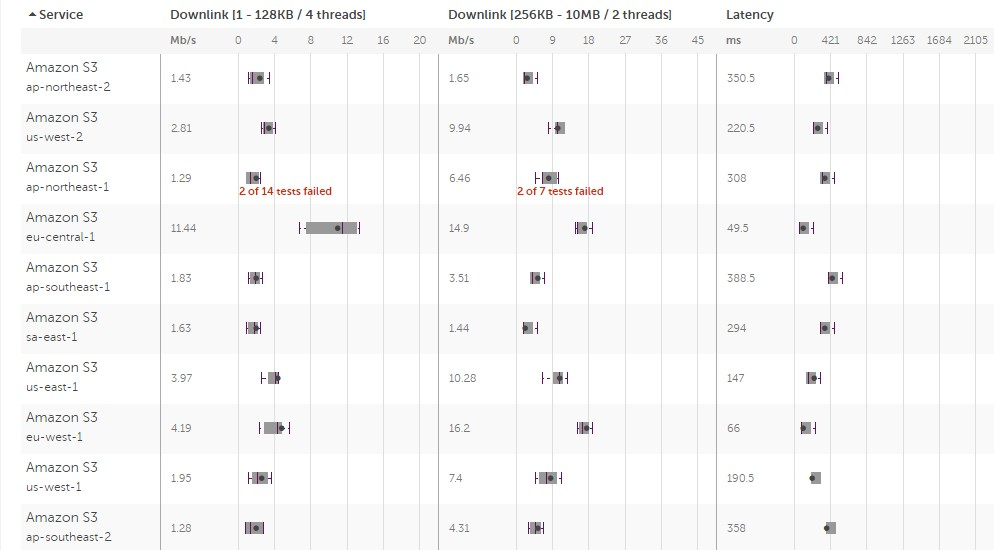
\includegraphics[width=14cm]{Img/AmazonS3.jpg}
        \caption{Amazon S3 CloudHarmony benchmark rezultat.}
        \label{fig:ch1}
    \end{center}
\end{figure}

\begin{figure}[H]
    \begin{center}
        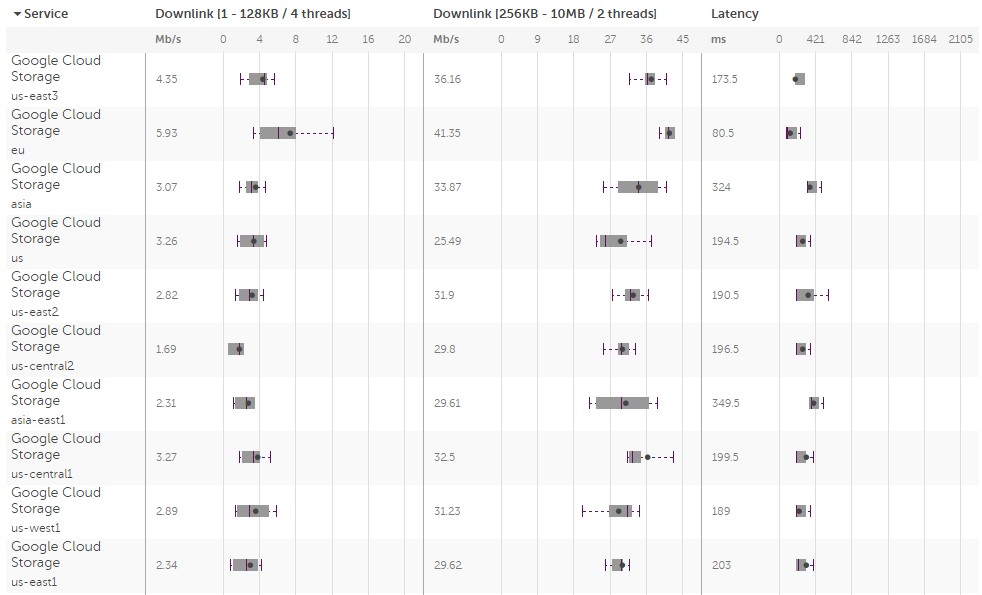
\includegraphics[width=14cm]{Img/GoogleStorage.jpg}
        \caption{Google Cloud Storage CloudHarmony benchmark rezultat.}
        \label{fig:ch2}
    \end{center}
\end{figure}

\begin{figure}[H]
    \begin{center}
        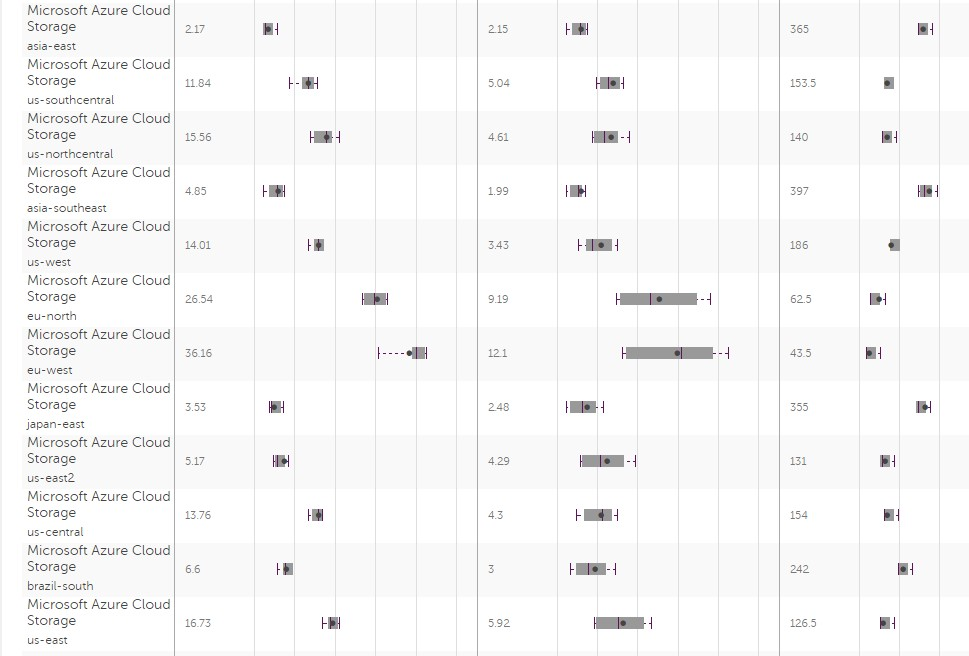
\includegraphics[width=15cm]{Img/MicrosoftAzure.jpg}
        \caption{Microsoft Azure CloudHarmony benchmark rezultat.}
        \label{fig:ch3}
    \end{center}
\end{figure}

Pri Amazon S3 je iz škatel z brki (angl. \textit{box plot}) razvidno, da je downlink najhitrejši na eu-central strežniku. Ista zgodba je tudi pri latenci, najnižja je v centralni Evropi (glej sliko \ref{fig:ch1}).

Google Cloud Storage ima v Evropi samo en strežnik, in sicer na zahodu. Tudi ta je najhitrejši po odzivnosti in prenosu podatkov glede na ostale kontinente (glej sliko \ref{fig:ch2}).

Zadnji je še Microsoft Azure, pri katerem ponovno prevladuje evropski strežnik, je bilo pa velika podobnost med Severno in Zahodno Evropo. Po večjem številu testov je prevladal zahod (glej sliko \ref{fig:ch3}).

Za vse tri ponudnike je očitno, da imajo najhitrejše in najodzivnejše strežnike v Evropi. Pričakovali smo, da pri vseh treh do tega ne bo prišlo, ker se ponavadi pretakajo informacije po celemu svetu, a očitno ima geografska razdalja večji vpliv kot smo mislili. Ob kratkem pregledu na internetu smo ugotovili \cite{serverdistance}, da je odvisno kje je postavljen naš ISP (angl. \textit{Internet service provider}) oz. v tem primeru CloudHarmony strežnik, ki izvaja teste. Očitno je CloudHarmony testni strežnik lociran nekje v Evropi in ker smo geografsko tudi mi najbližji ponudnikom v Evropi, smo se dokončno odločili za zgoraj navedene lokacije.

Ob kategoričnem pregledu rezultatov je Microsoft Azure z najkrajšo latenco in največjim downlinkom zmagovalec na izbranem benchmarku.
Drugo mesto je zasedel Google. Njegov downlink se zelo približa Microsoftovemu, a je latenca podvojena.
Amazonova latenca je malo večja od Azure-a, vendar je downlink približno dvakrat manjši kot pri ostalih dveh ponudnikih.\\

Uplinka in DNS-ja kljub možnosti izbire ni bilo mogoče testirati, saj očitno CloudHarmony pri teh storitvah tega ne podpira. Predpostavili pa smo, da so hitrosti za uplink glede na lokacijo podobne downlinku.

\section{Lastni testi} \label{lastni_testi}
Naši lastni testi so usmerjeni v čas upload-a in download-a posamezne storitve. Opravili smo več različnih testov, vsakega s svojim določenim tipom bremena, kjer smo za vsak test ločili bremena glede na posamezno lastnost (velikost datoteke, tip datoteke, število datotek, itd.)
\newline
Testirali smo torej upload/download čas:
\begin{itemize}
    \item posamezne datoteke,
    \item večih datotek,
    \item datotek različnih velikosti,
    \item datoteke pred vstavitvijo in po vstavitvi v predpomnilniku na oblaku,
    \item \ldots
\end{itemize}
Za dostop in testiranje storitev smo uporabljali unix-ov terminal, v katerem se avtomatizirano izvaja \textit{bash} skripta.
\newline
Za posamezno storitev smo uporabili naslednja bash orodja:
\begin{itemize}
    \item \texttt{azure cli} za Microsoft Azure \cite{azure_cli},
    \item \texttt{gsutil} za Google Cloud Storage \cite{gsutil},
    \item \texttt{aws cli} za Amazon S3 \cite{aws_cli}.
\end{itemize}


\subsection{Breme}
Z določitvijo bremena smo testirali latenco in odzivnost ponudnika - za sekvenčno ter paralelno prenašanje. Glede na pridobljene rezultate smo poskušali ugotoviti ali uporabljajo \textit{cache} (za majhne datoteke) in kompresijo (za določen tip datoteke, velike datoteke, itd.). Poskušali smo se izogniti zunanjim vplivom in pridobiti čimbolj pristne rezultate. Meritve smo zato izvedli večkrat - vsako uro, tekom enega dneva - a smo bili s številom testiranj omejeni, ker se poslužujemo brezplačne verzije pri vseh ponudnikih. 
Testiranje smo izvajali na sledečih bremenih:

\begin{multicols}{2}
\begin{itemize}
    \item Posamezne datoteke:
        \begin{itemize}
            \item 1kB,
            \item 10kB,
            \item 100kB,
            \item 1MB,
            \item 10MB,
            \item 100MB,
            \item 500MB,
            \item 1GB.
        \end{itemize}
    \item Več datotek:
        \begin{itemize}
            \item 1kB   x 2, 5, 10, 50, 100,
            \item 10kB  x 2, 5, 10, 50, 100,
            \item 100kB x 2, 5, 10, 50, 100,
            \item 1MB   x 2, 5, 10, 50, 100,
            \item 10MB  x 2, 5, 10, 50, 100,
            \item 100MB x 2, 5, 10,
            \item 500MB x 2, 5,
            \item 1GB   x 2.
        \end{itemize}
\end{itemize}
\end{multicols}

Testne datoteke so končnice \textit{.txt}, napolnjene z naključnimi podatki. Za testiranje download/upload pri načinu ''več datotek'' potrebujemo pripravljeno okolje in sicer smo zgradili drevesno strukturo datotek. V korenskem imeniku se nahajajo sinovi, ki so razdeljeni po velikosti datotek, ki jih vsebujejo. Znotraj so datoteke istih velikosti razdeljene še po kvantiteti, torej vsak imenik vsebuje število datotek, ki se bo paralelno preneslo. \\
Za ustvarjanje in kopiranje datotek smo uporabili skripto \ref{skripta1}. \\

\begin{lstlisting}[language=bash, captionpos=b, caption={Skripta za ustvarjanje in kopiranje datotek.}, label={skripta1}]
#!/bin/bash

SIZE=$1
NUMBER=$2
PREFIX=$3
DESTINATION=$4

# Ustvarjanje tekstovne datoteke poljubne velikosti
base64 /dev/urandom | head -c $SIZE  > $PREFIX.txt

# Kopiranje datoteke poljubno krat
for file in `seq 1 $NUMBER`; do
    filename=${PREFIX}_${file}
    cp $PREFIX.txt $DESTINATION/$filename.txt
done

# Odstranitev originalne datoteke
rm $PREFIX.txt
\end{lstlisting}

\subsection{Samodejno izvajanje testov}
Ker se izogibamo ročnemu poganjanju in beleženju rezultatov, smo napisali skripto \ref{skripta2}, ki bo to opravljala namesto nas. Skripte smo poganjali na \textit{eduroam} omrežju na serverju \textit{XeonPhi} (z dovoljenjem as. uni. dipl. ing. Davor Sluga), saj server teče 24/7, sploh pa bo zaradi 24-ih jeder in 64GB \textit{RAM}-a prenašanje datotek nemoteno. Obremenitev omrežja na žalost nismo mogli preveriti, ker na strežniku nimamo \texttt{sudo} (angl. kratica za \textit{superuser do}) pravic, da bi nameščali dodatna orodja, zato smo teste pognali večkrat in z izračunom povprečja ter standardne deviacije zmanjšali vpliv iregularnih rezultatov.
V primeru plačljivih verzij, bi za zanesljivejše rezultate testirali še na drugih omrežjih. Pri brezplačnemu načinu pa to ni možno, ker nam omejujejo število operacij, več računov pa ne moremo ustvariti, ker za registracijo zahtevajo številko kreditne kartice.\\

\begin{lstlisting}[language=bash, captionpos=b, caption={Skripta za samodejno izvajanje testov.}, label={skripta2}]
#!/bin/bash

printf "%s\n" "arguments:"
printf "%s\n" "-m ----> multiple files"
printf "%s\n" "-t ----> followed by int time in hours \
        (execute every H hours)"
printf "%s\n" "-n ----> execute N times"

SOURCE=single_files
H=1
N=24
S3Bucket=s3://zzrs2016mf/
GSbucket=gs://zzrs2016/
iter=0

while [ "$#" -gt 0 ]
do
	case $1 in
	-m)
		SOURCE=multiple_files
		shift 1
		continue
		;;
    -t)
        H=$2
        shift 2
        continue
        ;;
    -n)
        N=$2
        shift 2
        continue
        ;;
	*)
		;;
	esac
	shift
done

for iter in $(seq 1 $H);
do
    for map in $HOME/$SOURCE/*
    do
      for file in $map/*
      do
        ./amazonS3.sh -s $file -d $S3Bucket # upload
        ./amazonS3.sh -D  # download
        aws s3 rm --recursive $S3Bucket

        ./azure.sh -s $file 
        ./azure.sh -D 
        azure storage blob delete zzrs zzrs

        ./google.sh -s $file -d $GSbucket # upload
        ./google.sh -D
        gsutil rm $GSbucket**

        rm -rf ~/downloads/
      done
    done
  sleep $Hh
done

\end{lstlisting}

\subsection{Amazon S3}
Najprej smo na Amazonu ustvarili račun z osebnimi podatki in prestali avtorizacijo. Izbrali smo brezplačni paket, ki traja 12 mesecev. Ponudnik obljublja skalabilen in zanesljiv sistem z nizko latenco ter:
\begin{itemize}
    \item 5GB prostora,
    \item 20.000 \textit{GET} zahtev,
    \item 2.000 \textit{PUT} zahtev.
\end{itemize}

Sledila je kreacija \textit{bucketa} (odlagališče), dodelitev pravic (trenutno \textit{public}) in zapis \textit{credentionals} v \texttt{.bashrc} kot okoljske spremenljivke (\texttt{AWS\_ACCESS\_KEY\_ID} in\\ \texttt{AWS\_SECRET\_ACCESS\_KEY}). \\
S pomočjo \textit{AWS CLI} (angl. \textit{Command Line Interface}) ukaza smo napisali skripto \ref{skripta3}, ki obdela argumente in jih posreduje aws-ju, medtem pa meri čas izvajanja uploada ali downloada. Za prenos in pošiljanje se uporablja bash komande \texttt{cp}, kjer samo zamenjujemo izvor (angl. \textit{source}) in cilj (angl. \textit{destination}) za željeno operacijo (download/upload). S stikalom \texttt{--recursive} prenašamo celotne imenike, avtor \textit{API}-ja (angl. \textit{Application programming interface}) pa nam zagotavlja, da se prenašanje izvaja paralelno.\\

\begin{lstlisting}[language=bash, captionpos=b, caption={Skripta za testiranje Amazon S3 storitve.}, label={skripta3}]
#!/bin/bash

printf "%s\n" "arguments:"
printf "%s\n" "-s ----> source file (path)"
printf "%s\n" "-d ----> destination file (path)"
printf "%s\n" "-D ----> download (upload is the default\
        action)"

DESTINATION=s3://zzrs2016/test
SOURCE=upload_test
UPLOAD=upload
HOME=~/downloads/

while [ "$#" -gt 0 ]
do
    case $1 in
    -s)
	    SOURCE=$2
	    shift 2
	    continue
	    ;;
    -d)
    	DESTINATION=$2
    	shift 2
    	continue
    	;;
    -D)
    	UPLOAD=download
    	SOURCE=s3://zzrs2016mf/
    	;;
    *)
	    ;;
    esac
    shift
done

   timestamp=$( date +"at: %d-%m-%Y %H:%M:%S" )
   START=`date +%s%N`
   
   if [[ $UPLOAD == "upload" ]]
   then
     aws s3 cp $SOURCE $DESTINATION --recursive --quiet 
   else
     aws s3 sync $SOURCE $HOME --quiet
   fi
   
   END=`date +%s%N`
   ELAPSED=`echo "scale=5; \ 
            $(($END - $START)) / 1000000000" | bc`
   echo "File: $SOURCE, Started $UPLOAD" \
        "$timestamp, lasted: [$ELAPSED] seconds." \
         >> "rezultatiAmazonS3.txt"

\end{lstlisting}

\subsection{Google Cloud Storage}
Pri GCS je brezplačna ponudba malo drugačna. Ob registraciji so nam dali \textbf{300\$} virtualnega denarja, ki ga lahko mirne vesti zapravljamo na njihovi strani. Cene storitev, ki smo jih uporabljali, so sledeče:
\begin{itemize}
    \item \textbf{\$0.10} na 10.000 operacij za \textit{GET} ali \textit{PUT} ukaze,
    \item Standard storage (tip bucketa, najnižja latenca) \textbf{\$0.026} na GB podatkov na mesec,
    \item \textit{DELETE} je brezplačen.
\end{itemize}
Lokalni terminal smo z bucketom povezali preko ukaza \texttt{gsutil config}. Ta nam vrne \textit{url} (angl. \textit{Uniform Resource Locator}) naslov na katerem dobimo aktivacijsko kodo, ki jo nato vpišemo v terminal. \\

Skripta za prenašanje datotek je sila podobna Amazonovi, saj za prenos tudi uporablja ukaz \texttt{cp}. S kombinacijo stikal \texttt{-r} (\textit{recursive}) prenašamo imenike,  z \texttt{-m} pa paralelno prenašanje.
Primer uporabe: \texttt{gsutil -m cp -r dir gs://zzrs}. Skripte zaradi podobnosti ne bomo prilagali.

\subsection{Microsoft Azure}
Azure CLI nam prav tako ponuja širok spekter ukazov s katerimi delamo na Azure platformi, kjer je velik poudarek na operiranju z \textit{Blobi}. Za dostopanje do storitve smo najprej kreirali uporabniški račun in ob registraciji dobili \textbf{200\$} virtualnega denarja, ki se troši s hranjenjem in prenašanjem datotek (blobov). Cene storitev, ki smo jih uporabljali, so sledeče:
\begin{itemize}
    \item za \textit{Standard storage (Block blobs)} na mesec za prvi TB podatkov hranjenje stane \textbf{\$0.024} na GB podatkov,
    \item na 100.000 transakcij (branje/pisanje) je \textbf{\$0.0036} tarife,
    \item brisanje je brezplačno.
\end{itemize}
Že takoj opazimo, da je ta storitev cenovno najugodnejša in je ne glede na odzivnost storitve najboljša izbira za uporabnika, ki hoče koristiti brezplačno verzijo. \\  

Po registraciji smo se preko terminala povezali na \textit{container} tako, da smo se najprej indentificirali z vključitvijo \texttt{AZURE\_STORAGE\_ACCOUNT} in
\texttt{AZURE\_STORAGE\_ACCESS\_KEY} v datoteko \texttt{.bashrc}. Za sam prenos datotek nam je spet ponujen intuitiven \textit{API}, a se od ostalih dveh ponudnikov ločuje z uporabo dveh različnih funkcij za upload in download. Primer uporabe:\\
\texttt{azure storage blob upload source\_to\_upload container\_name blob\_name}.\\
\texttt{azure storage blob download container\_name blob\_name destination\_folder}.\\

Značilnost tega ponudnika je, da se podatki prenašajo v \textit{blob-ih}. Azure blob je storitev za shranjevanje velike količine nestrukturiranih podatkov, kot so besedilo ali binarni podatki, do katerih lahko dostopamo prek HTTP ali HTTPS. Na sliki \ref{fig:blob} je razvidno, kakšno arhitekturo uporablja Azure.
\begin{figure}[H]
    \begin{center}
        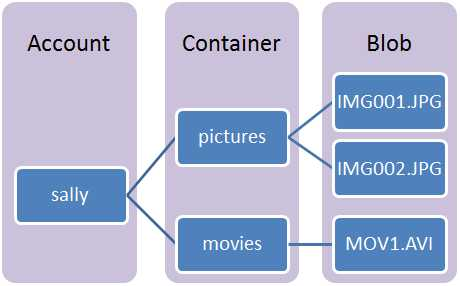
\includegraphics[width=6cm]{Img/blob.jpg}
        \caption{Primer Azure Blob storitve.}
        \label{fig:blob}
    \end{center}
\end{figure}
Obstajajo tri vrste blob-ov: \textit{block blobs}, \textit{page blobs} in \textit{append blobs}. Block blobs so namenjenji hranjenju tekstovnih in binarnih datotek (npr. dokumenti, medijske datoteke, itd.). Append blobi se uporabljajo za isti namen, razlika je le, da so sestavljeni iz blokov in so optimizirani za hitro dodajanje (uporablja se jih lahko npr. za logiranje). Page blobi so namenjeni za večje datoteke (do 1 TB) in so uporabni, kadar potrebujemo hitre dostope za branje/pisanje. Ker uporabljamo brezplačno verzijo in imamo omejene kredite, uporabljamo Block blobe, saj ne bomo prenašali ogromnih datotek, poleg tega pa so tudi tekstovne narave. \\

Struktura napisane skripte se je ohranila v primerjavi z ostalima dvema, razlikujejo se le ukazi za prenos datotek. Nažalost pa to orodje in ostale alternative ne ponujajo sočasnega prenašanja večjega števila datotek, zato smo pri Microsoft Azure testirali in primerjali samo rezultate za prenašanje ene datoteke naenkrat.

\subsection{Primerjava rezultatov}

Pri testiranju za eno datoteko naenkrat smo izvedli 24 iteracij za vse 3 ponudnike naenkrat in enournim razmakom med iteracijami. Pri testiranju za več datotek (paralelni prenos) naenkrat pa smo zaradi omejenih resursov izvedli 12 iteracij z dvournim razmakom samo za Google in Amazon, ker Azure ne podpira paralelnega prenosa.
Prav tako je vredno omeniti, da smo teste izvajali čez vikend, ker je po analizi lanske 6. skupine \cite{6_skupina} takrat obremenitev strežnika Amazon S3 v Evropi najmanjša. Enako smo predpostavili za ostala dva ponudnika.

Za vse iteracije smo izračunali povprečje prenosa, ker pa smo nekajkrat dobili iregularne rezultate, smo vključili v izračun tudi standardno deviacijo.

\subsubsection{Testiranje enkratnega prenosa}

Na sliki \ref{fig:graph1} za download se takoj opazi, da so jasni hitrostni pasovi za vse tri ponudnike, ne glede na velikost datoteke. Najhitrejši je Amazon, drugi Google in tretji Azure. Uvrstitev je ravno obratna kot pri CloudHarmony (glej poglavje \ref{cloudharmony}), a težko ugotovimo kje in zakaj je do tega prišlo, ker na njihovi strani ne opisujejo prav posebej kako in kakšne teste izvajajo. Je pa zanimivo, da je uvrstitev skladna z radodarnostjo ponudbe za brezplačno verzijo. Amazon nudi najmanj, a to opravi z največjo hitrostjo, Google ima srednjo drago storitev ter srednjo hitrost, Azure pa ponuja najcenejšo storitev, a se to odraža tudi v hitrosti prenosa. 

Pri vseh treh ponudnikih je za downloadiranje vidno, da je čas prenosa do velikosti 10000kB skoraj zanemarljiv in do izraza pride le latenca, ki pa med ponudniki raste v enakem zaporedju kot sam download. Za velike datoteke (nad 100000kB) čas prenosa raste precej linearno, torej nobeden ne uporablja kompresije ali pa paralelnega prenosa po koščkih. Googlova krivulja se po obliki prilagaja Azurovi in za velike datoteke obe strmo naraščata, medtem, ko pri Amazonu narašča z manjšim naklonom in za 1GB veliko datoteko prinaša že do 50 sekund razlike v prenosu.

\begin{figure}[H]
    \begin{center}
        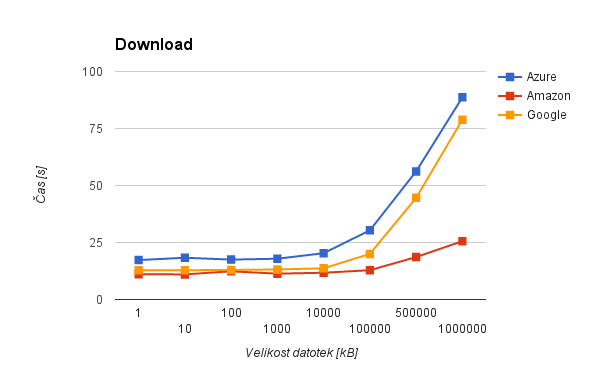
\includegraphics[height=7.7cm]{Img/sf_download_avg.png}
        \caption{Graf povprečnega downloada ene datoteke.}
        \label{fig:graph1}
    \end{center}
\end{figure}

Do odstopanj pri Azure-u in Amazonu (glej sliko \ref{fig:graph2}) pride le za manjše datoteke, pri večjih pa se je čas prenosa večinoma držal povprečja. Pri Googleu pa je bilo ravno obratno, za manjše datoteke je bila standardna deviacija izredno majhna, medtem ko je za velike datoteke (nad 10000kB) eksponentno naraščala. To nakazuje na izredno nestabilno storitev, a mogoče smo imeli le smolo in naleteli na obdobje vzdrževalnega dela na serverju. 

\begin{figure}[H]
    \begin{center}
        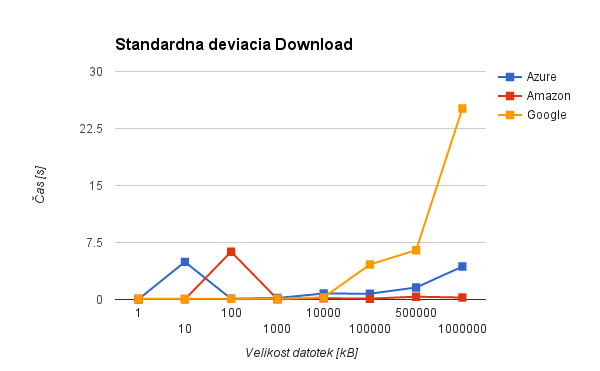
\includegraphics[height=8.5cm]{Img/sf_download_stddev.png}
        \caption{Graf standardne deviacije downloada ene datoteke.}
        \label{fig:graph2}
    \end{center}
\end{figure}

Za upload je s slike \ref{fig:graph3} razvidna drugačna razvrstitev. Na prvem mestu je še vedno Amazon, sta se pa zamenjala Google in Azure. Med ponudniki in njihovimi krivuljami uploada glede na velikost datoteke ni več očitnih podobnosti, pač pa vsaka narašča s svojim naklonom. Prav tako je razlika med ponudniki večja za upload kot za download, torej imata Azure in Google pred sabo še precej optimizacije za nalaganje datotek.

Prag latence za Azure ostaja pri do 10000kB, pri Googleu in Amazonu pa so večje časovne razlike opazne že za datoteke večje od 1000kB. Tudi tukaj je razvidno, da sta hitrost uploada in višina latence povezana, torej nobena storitev ne potrati preveč časa za rokovanje (angl. \textit{handshake}).

\begin{figure}[H]
    \begin{center}
        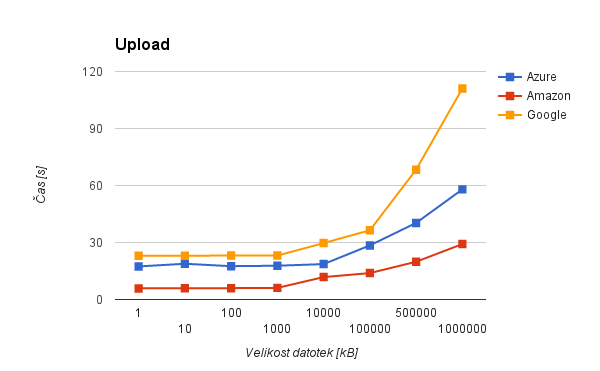
\includegraphics[height=7cm]{Img/sf_upload_avg.png}
        \caption{Graf povprečnega uploada ene datoteke.}
        \label{fig:graph3}
    \end{center}
\end{figure}

Pri standardnem odklonu za upload (glej sliko \ref{fig:graph4}) se zgodba ponovi, nekaj manjših razlik je prišlo pri Azureu, Google pa je ponovno variiral za velike datoteke (nad 100000kB). Konsistenca je pri prenašanju lahko izredno pomembna in se je vsekakor splačalo izvesti teste večkrat, ker smo le tako dobili bolj točno oceno ponudnikov. Če bi imeli neomejeno resursov, bi seveda testirali večkrat v enem tednu in mogoče dobili lepše rezultate (manj deviacije), ampak razvrstitev ponudnikov bi verjetno ostala kar ista.

\begin{figure}[H]
    \begin{center}
        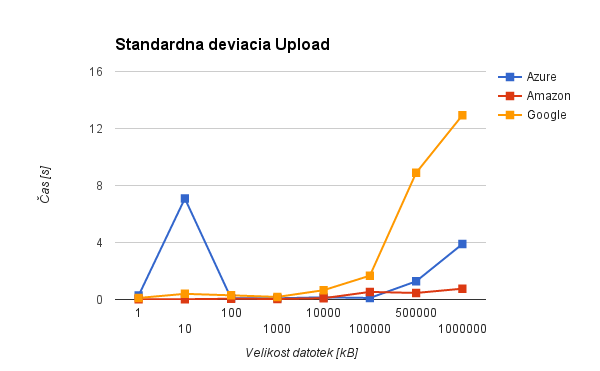
\includegraphics[height=7cm]{Img/sf_upload_stddev.png}
        \caption{Graf standardne deviacije uploada ene datoteke.}
        \label{fig:graph4}
    \end{center}
\end{figure}

Če pri download operaciji pogledamo najboljše primere testiranja za npr. 1GB datoteke (glej sliko \ref{fig:graph5}), lahko opazimo, da je Amazonov praktično enak kot povprečje, kar je precej presenetljivo, ker sta se za to breme ostala dva uporabnika izkazala precej slabše. Pri Azure je najboljši primer le za nekaj sekund hitrejši od povprečja. Googlov najboljši primer pa se zelo razlikuje od povprečja, in sicer kar za dobrih 50 sekund. To je znova dokaz Googlove nekonsistentnosti, ki se izraža tudi pri najslabšem primeru.

Za najslabše primere download testiranja za 1GB velike datoteke na sliki  \ref{fig:graph6} opazimo, da je Amazon znova tik ob povprečju, kar glede na najboljši primer ni presenečenje. Azure je nekoliko slabši, ampak še vseeno ni tako daleč od povprečja (približno 10-15 sekund). Google je znova precej zgrešil povprečje. Ker smo teste opravljali čez vikend (zaradi manj prometa - ugotovitev lanske 6. skupine \cite{6_skupina}, težko določimo razlog za tako veliko odstopanje. Mogoče so takrat opravljali kakšna vzdrževalna dela na strežniku, ali pa je to posledica kakšnega drugega dogodka na katerega nismo računali. Dodatna možna razlaga je, da Google enostavno ponuja nekonsistenten sistem za svoje brezplačne storitve in je mogoče stanje pri plačljivi verziji drugačno. Standardna deviacija močno potrjuje naš sklep o Googlovi nezanesljivosti.

\begin{figure}[H]
    \begin{center}
        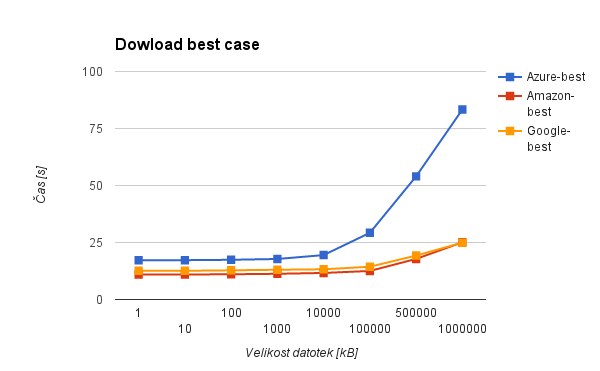
\includegraphics[height=8.5cm]{Img/dBest.png}
        \caption{Graf najboljših primerov download-a.}
        \label{fig:graph5}
    \end{center}
\end{figure}
\begin{figure}[H]
    \begin{center}
        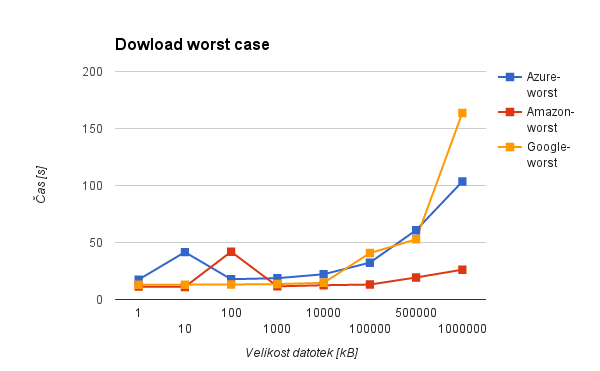
\includegraphics[height=8.5cm]{Img/dWorst.png}
        \caption{Graf najslabših primerov download-a.}
        \label{fig:graph6}
    \end{center}
\end{figure}

Pri najboljših primerih upload operacije (glej sliko \ref{fig:graph7}) za datoteke velike 1GB, lahko pri vseh potegnemo enake ugotovitve kot pri najboljših primerih download operacije. Trend se že ves čas ponavlja. Amazon zelo konsistenten, Azure malo manj, Google zelo nekonsistenten.

Za najslabše primere upload operacije (glej sliko \ref{fig:graph8}) lahko prav tako opazimo podobnost z našo analizo najslabših primerov download operacije. Tukaj lahko potegnemo končno črto, da Googlova storitev enostavno ne ponuja zanesljivosti, saj je enako kot pri download operaciji tudi tukaj standardna deviacija ogromna v primerjavi z Azure in Amazon. To nam pokažeta tudi najboljši in najslabši čas Googlovega uploada, saj se razlikujeta za dobrih 50 sekund.

\begin{figure}[H]
    \begin{center}
        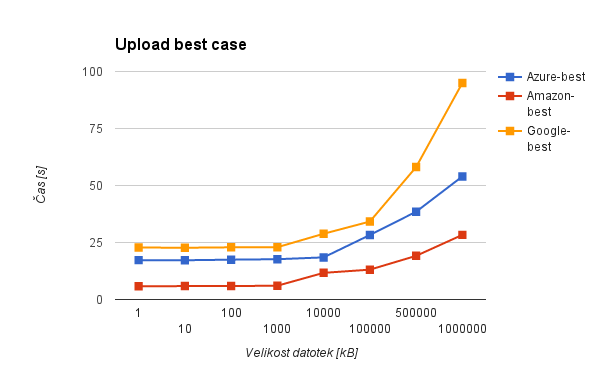
\includegraphics[height=8.5cm]{Img/uBest.png}
        \caption{Graf najboljših primerov upload-a.}
        \label{fig:graph7}
    \end{center}
\end{figure}
\begin{figure}[H]
    \begin{center}
        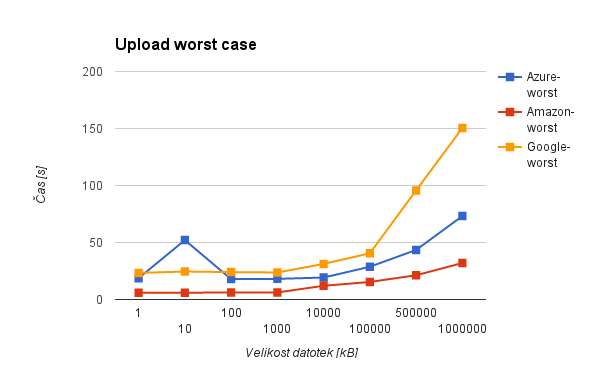
\includegraphics[height=8.5cm]{Img/uWorst.png}
        \caption{Graf najslabših primerov upload-a.}
        \label{fig:graph8}
    \end{center}
\end{figure}

\subsubsection{Testiranje paralelnega prenosa}

Najprej smo izvedli testiranje na eni datoteki naenkrat, zato smo ob pričetku testiranja paralelnega prenosa postavili hipotezo, da bo Amazon ponovno prevzel vodstvo in smo predvidevali da bo čas prenosa linearno naraščal s številom datotek.
Za konec smo naredili še analizo vseh paralelnih testov skupaj, ker nas je zanimalo, koliko bi to vplivalo na časovno skalo. 
Tudi pri paralelnemu prenosu se je izkazalo, da je Amazon hitrejši od Googla, kar pomeni da smo potrdili prvi del hipoteze.\\

Pri povprečnem downloadu večih datotek (glej sliko \ref{fig:graph9}), nas je Amazon presenetil z skoraj vodoravno krivuljo ne glede na velikost. Tukaj je najverjetneje problem pri \textit{AWS CLI} orodju in ukazu \texttt{sync} \cite{sync}.\\
\begin{figure}[H]
    \begin{center}
        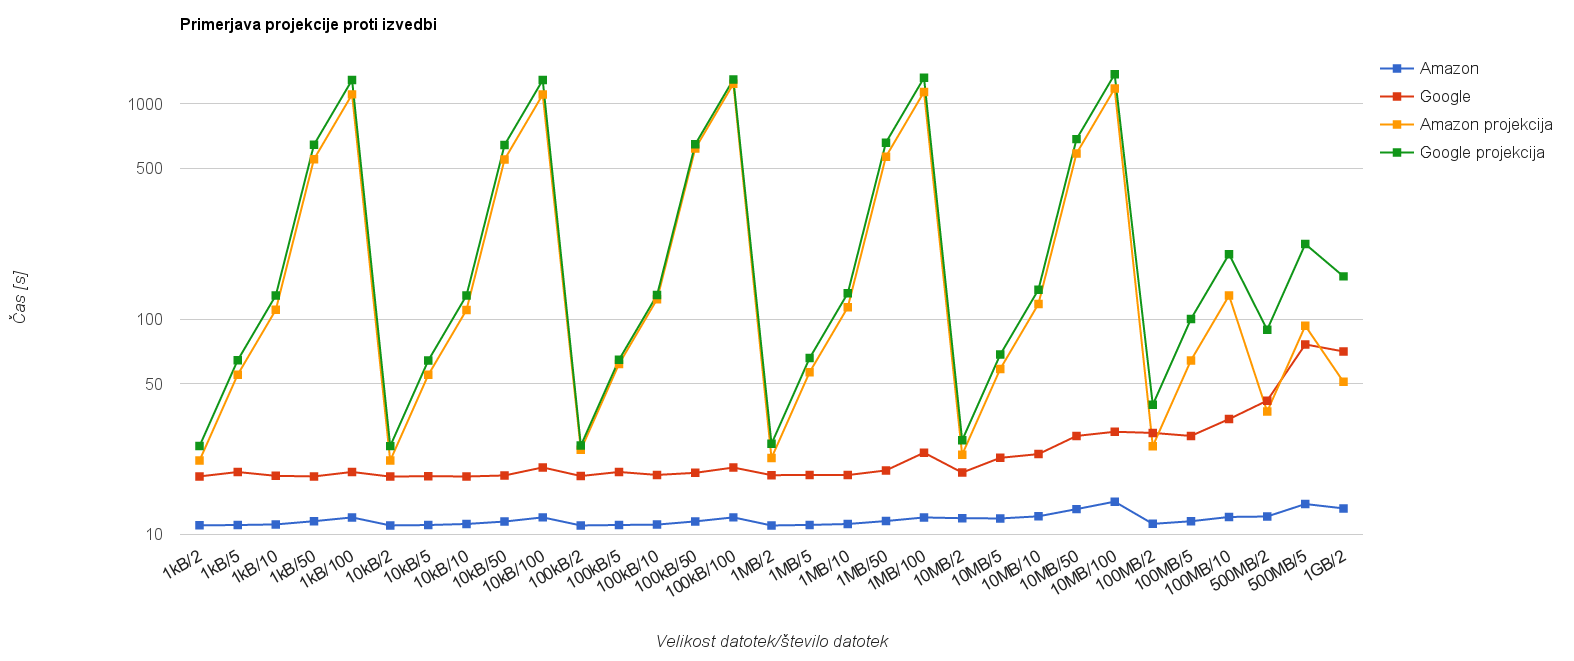
\includegraphics[width=17cm]{Img/projekcijaVSizvedbaDown.png}
        \caption{Graf povprečnega downloada večih datotek naenkrat in napoved rezultatov.}
        \label{fig:graph9}
    \end{center}
\end{figure}

Pri standardni deviaciji za download večih datotek (glej sliko \ref{fig:graph10}), ponovno pride do izraza nekonsistentnost download časov Googla, podobno kot pri testih enkratnega prenosa. Medtem, ko lahko pri Amazonu opazimo kako enovit je bil download čas ukaza \texttt{sync} in odstopanja praktično ni.

\begin{figure}[H]
    \begin{center}
        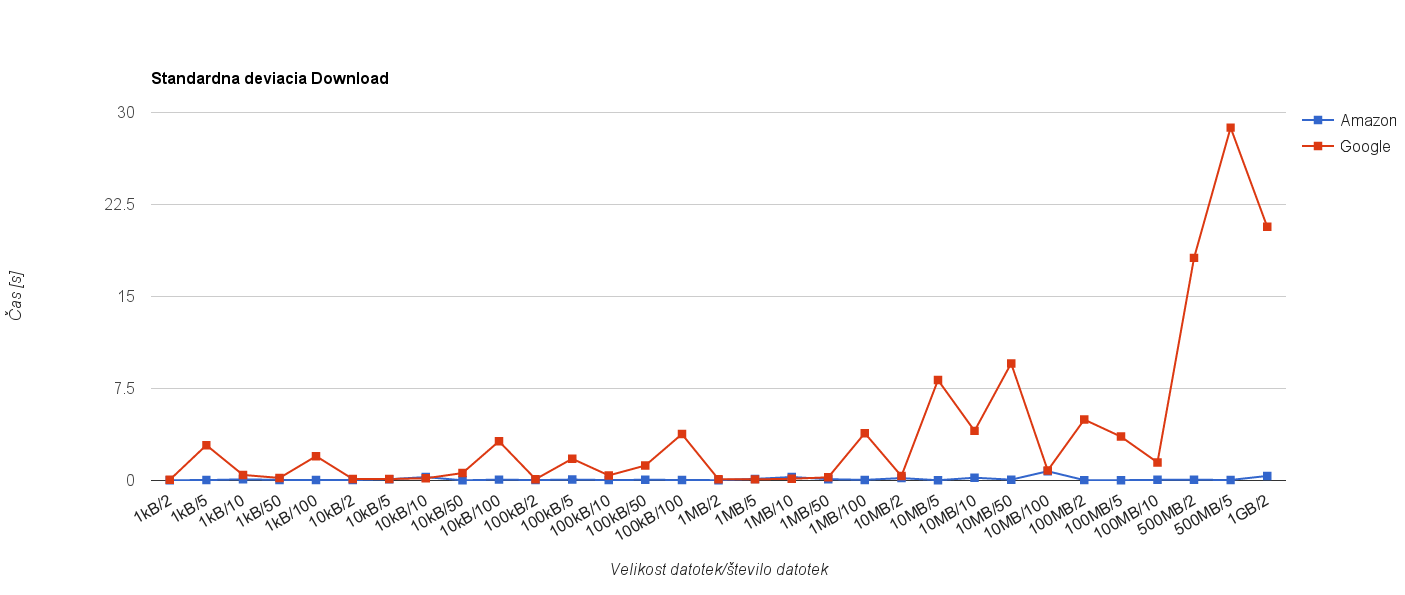
\includegraphics[width=16cm]{Img/mf_download_stddev.png}
        \caption{Graf standardne deviacije downloada večih datoteke naenkrat.}
        \label{fig:graph10}
    \end{center}
\end{figure}

Pri testiranju drugega dela hipoteze (linearna povezanost med časom in številom datotek) se je izkazalo, da oba ponudnika izkoriščata paralelni prenos. Iz slike \ref{fig:graph11} je razvidno da naša predpostavka o sekvenčnem prenosu ne drži, pravzaprav naši ponudniki svoje delo opravljajo mnogokrat hitreje kot smo napovedali.

\begin{figure}[H]
    \begin{center}
        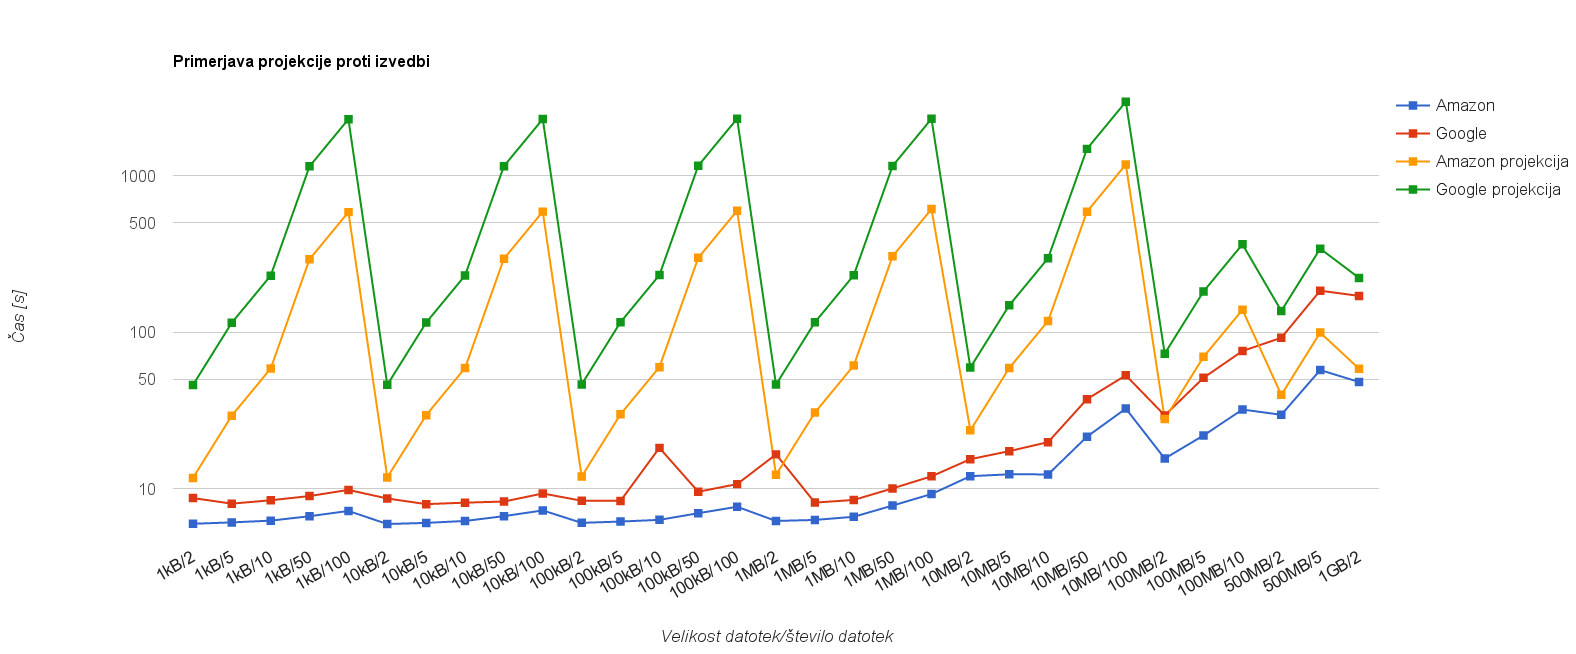
\includegraphics[width=16cm]{Img/mf_upload_avg_projection.png}
        \caption{Graf povprečnega uploada večih datotek naenkrat in napoved rezultatov.}
        \label{fig:graph11}
    \end{center}
\end{figure}

Zgodba se pri standardni deviaciji uploada večih datotek ponovi (glej sliko \ref{fig:graph12}), saj spet pride do nihanj pri Googlovi storitvi. Pri Amazonu je do malo večjega odstopanja prišlo le pri večjih datotekah, a le pri večjem številu uploadanih datotek.

\begin{figure}[H]
    \begin{center}
        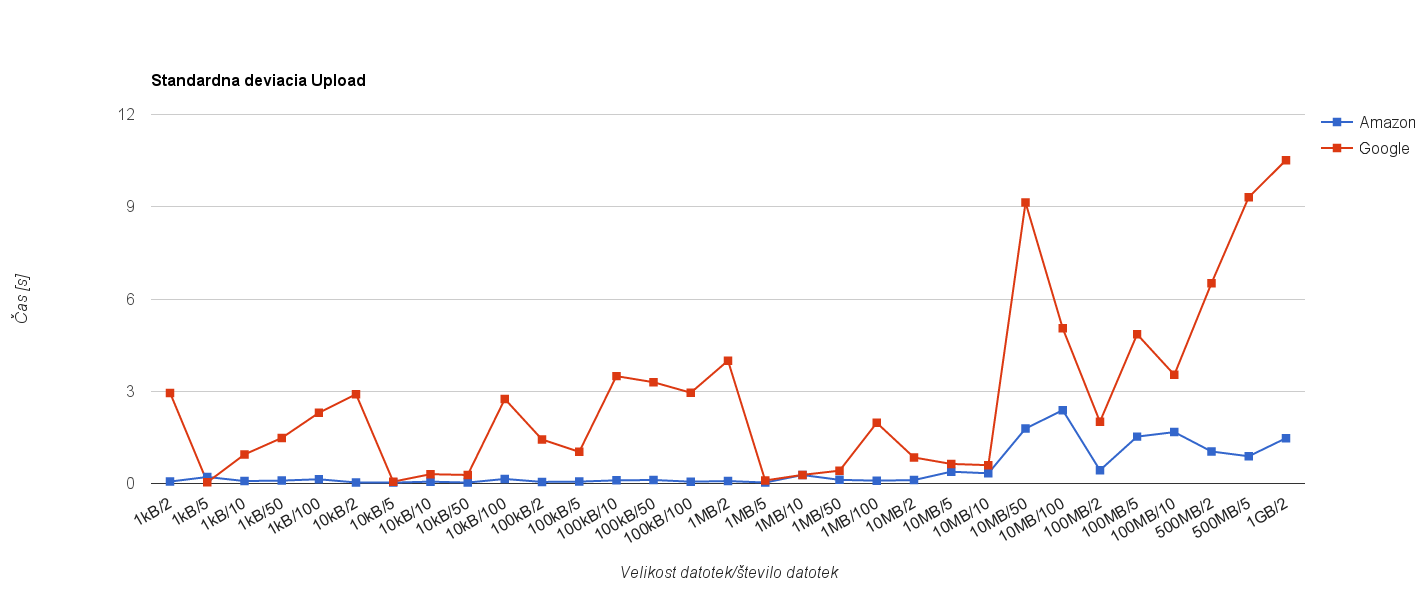
\includegraphics[width=16cm]{Img/mf_upload_stddev.png}
        \caption{Graf standardne deviacije uploada večih datoteke naenkrat.}
        \label{fig:graph12}
    \end{center}
\end{figure}

\subsubsection{Metrika zmogljivosti}
Iz naših grafov in analiz je razvidno, da je ponudnik Microsoft Azure performančno najbolj povprečen ter cenovno najugodnejši, zato smo se odločili, da se za analizo metrike zmogljivosti osredetočimo le na tega ponudnika. 

Merili smo čas prenosa datoteke med oblakom ter uporabnikom, ki ga lahko predstavimo z enačbo \(T = T_{1} + T_{2} + T_{3}\). Sestavljajo jo sledeči parametri:
\begin{itemize}
    \item \(T_{1}\): čas dostopa do storitve,
    \item \(T_{2}\): čas procesiranja zahteve,
    \item \(T_{3}\): čas prenosa datoteke med oblakom in uporabnikom (upload / download).
\end{itemize}
Za testna bremena smo vzeli enake datoteke kot pri ostalih testiranjih in za njih izmerili povprečni čas prenosa v obeh smereh.

\(T_{1}\) smo v grobem ocenili glede na povprečno latenco, ki smo jo dobili iz Microsoft Azure CloudHarmony benchmark rezultatov (glej sliko \ref{fig:ch3}). Rezultat je bila izredno majhna vrednost in sicer \(T_{1} = 43.5ms\). Bolj bi bilo zanesljivo, če bi čas latence pridobili sami, a Azure zaradi strožje varnosti ne odgovarja na \textit{ICMP} (angl. \textit{Internet Control Message Protocol}) pakete, zato smo tukaj prisiljeni zaupati CloudHarmony-ju.

Pri prenosu datotek nam ponudnik pošlje oceno časa \(T_{3}\). Ker lahko merimo le skupni čas \(T_{D}\) (download) in \(T_{U}\) (upload), smo  morali izračunati čas \(T_{2}\) po enačbi \(T_{2} = T - (T_{1} - T_{3}) \). Iz grafov na sliki \ref{fig:graph13} in \ref{fig:graph14} je razvidno, da sta časa \(T_{1}\) in \(T_{2}\) bolj ali ne konstantna, medtem, ko čas \(T_{3}\) pri povečevanju velikost datotek (a šele pri 100MB) eksponentno narašča. 

\begin{figure}[H] 
    \begin{center}
        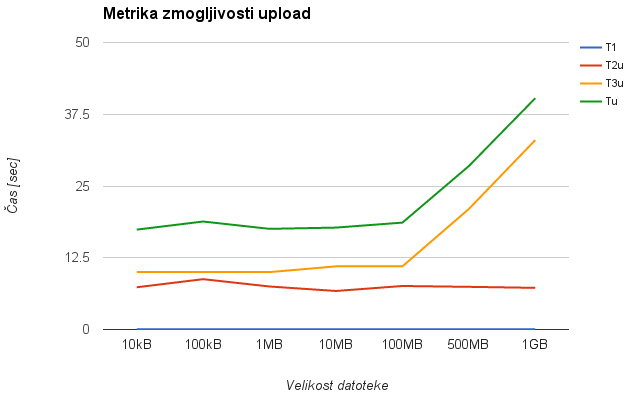
\includegraphics[width=10.5cm]{Img/metrika_upload.png}
        \caption{Graf metrike zmogljivosti za upload}
        \label{fig:graph13}
    \end{center}
\end{figure}

\begin{figure}[H]
    \begin{center}
        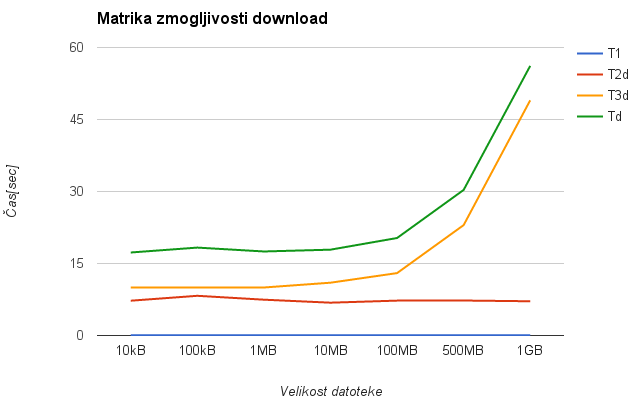
\includegraphics[width=10.5cm]{Img/metrika_download.png}
        \caption{Graf metrike zmogljivosti za download}
        \label{fig:graph14}
    \end{center}
\end{figure}

\section{Zaključek}
Iz vseh rezultatov testiranja je jasno razvidno, da je Amazon vsekakor na prvem mestu, kar se tiče hitrosti. Za uporabnika, ki pri oblačnih storitvah za hranjenje podatkov potrebuje predvsem hitrost in časovno konsistentnost, denar pa ni ovira, je prava izbira Amazon. Če pa nam je vseeno, koliko časa se datoteke prenašajo, ampak nas zanima samo koliko časa lahko storitev uporabljamo brezplačno, potem bi izbrali Azure, ki je najbolj radodaren z brezplačno verzijo. 

Vsekakor bi lahko našo raziskavo zelo izboljšali, če bi razširili število ponudnikov (DropBox, Mega, ...) in pognali več raznolikih testov. Zanimivo bi pa bilo poizkusiti tudi plačljive verzije, ker vsi trije ponudniki ponujajo hitrejše opcije prenosa, a seveda z večjo tarifo.


\bibliographystyle{unsrt}
\bibliography{literature.bib}

%\section{Viri}
%\begin{enumerate}
%  \item https://cloudharmony.com/ \label{cloudharm}
%  \item https://azure.microsoft.com/en-us/documentation/articles/storage-azure-cli/ \label{azure_cli}
%  \item https://cloud.google.com/storage/docs/gsutil \label{gsutil}
%  \item https://aws.amazon.com/cli/ \label{aws_cli}
%  \item http://serverfault.com/questions/346906/effect-of-distance-from-server-on-page-load-speed %\label{serverdistance}
%  \item http://lrss.fri.uni-lj.si/sl/teaching/zzrs/lectures/Recenzije/Sk\_6\_8.pdf \break[Dostopno: %02.05.2016] \label{6_skupina}
%  \item http://docs.aws.amazon.com/cli/latest/reference/s3/sync.html \label{sync}
%\end{enumerate}

\end{document}
